\documentclass[mathserif,10pt]{beamer}

\usepackage{beamerthemesplit}
\usepackage{graphics}
\usepackage{epsfig}
\usepackage{algorithm}
\usepackage{verbatim}
\usepackage{listings}
\usepackage{framed}
\usepackage{pstricks}
\usepackage{pst-node,pst-tree}
\usepackage{pst-rel-points}
\usepackage{flexiprogram}
\usepackage[UKenglish]{babel}
\usepackage{hyperref}
\usepackage{pst-coil}
\usepackage{color}
\usepackage{epsfig}
%\usepackage{tikz}
%\usepackage{multirow}

\usefonttheme{serif}

\newcommand{\cmt}[1]{}
%\noindent

\setcounter{tocdepth}{1}


\usepackage{color}
 
\definecolor{codegreen}{rgb}{0,0.6,0}
\definecolor{codegray}{rgb}{0.5,0.5,0.5}
\definecolor{codepurple}{rgb}{0.58,0,0.82}
\definecolor{backcolour}{rgb}{0.95,0.95,0.92}
\lstdefinestyle{mystyle}{
    %backgroundcolor=\color{backcolour},   
    commentstyle=\color{codegreen},
    keywordstyle=\color{magenta},
    %numberstyle=\tiny\color{codegray},
    stringstyle=\color{codepurple},
    basicstyle=\footnotesize,
    breakatwhitespace=false,         
    breaklines=true,                 
    captionpos=b,                    
    keepspaces=true,                 
    %numbers=left,                    
    %numbersep=5pt,                  
    showspaces=false,                
    showstringspaces=false,
    showtabs=false,                  
    tabsize=2
}
 
\lstset{style=mystyle,frameround=fttt}


\setbeamercovered{transparent=0}

  \usetheme{CambridgeUS}
  \usecolortheme{dolphin}

  \title[GRI]{GRI: \textbf{I}nterpreter of a dynamic language for \textbf{GR}aph algorithms}
  \author[]{{\textbf{Sandeep Dasgupta}} }
  \begin{document}

  \begin{frame}
  \titlepage
  \end{frame}
  \usebeamertemplate{mytheme}

  \AtBeginSection[]
{
  \begin{frame}<beamer>
    \frametitle{Outline}
  \tableofcontents[currentsection]
    \end{frame}
}

\defverbatim[colored]\lstdfs{
\begin{lstlisting}[language=C++,basicstyle=\tiny,keywordstyle=\color{red}]
  define("NUM_VERTICES", "10");
  define("NOTVISITED", "0");
  define("VISITED", "1");

  function dfs(v, dfsorder)
  {
      if(v.visit == VISITED)
        return;

      println("vertex visited: " + v.num);
      v.visit = VISITED;

      dfsorder.pushBack(v);

      foreach(neighbor; v.getNeighbors())
        dfs(neighbor, dfsorder);
  }

  function main(argv)
  {
    g = graph();
    g.loadFromFile(argv[0]);

    dfsorder = array(0);
    dfs(first, dfsorder);

    for(vertex: dfsorder ) {
      println(" " + vertex.__id + " " );
    }
  }

\end{lstlisting}
}

\defverbatim[colored]\lstsyntax{
\begin{lstlisting}[language=C++,basicstyle=\tiny,keywordstyle=\color{red}]
  //Supports arrays and array iterators
  arr = array(2);
  arr[0]  =  5;
  arr[1]  = "ABC";

  //Supports struct ans struct iterators
  arr = struct();
  arr.x  =  5;
  arr.y  = "ABC";

\end{lstlisting}
}

\section{Motivation}
\frame
{
  \frametitle{\secname}
  \begin{itemize}%[<+->]
    \item Graphical models are applied to widely varying fields.
    \begin{itemize}
      \item Biochemistry 
        \cmt{genomics}
      \item Electrical Engineering
        \cmt{communication networks }
      \item Computer Science
        \cmt{Algorithms and computation}
      \item Operations Research
        \cmt{Scheduling}
      \item Organizational Structures 
        \cmt{social networking}
    \end{itemize} 
    \vspace{1cm}
    \item Field experts often struggle to represent \& allow computations on  graphical models in \textbf{Convenient} and \textbf{Efficient} way.
      \cmt{
Convenience: is essential so that even for domain experts who are not coding experts
can code and reason about their implementation. Ease of interface could be due to:
– Expressive power of the language representing those models.
– Intuitive extensibility of the language.
– Ability of the language to provide exploratory programming, where the user may
experiment with different ideas (without dwelling much into the language syntax)
before coming to a conclusive one.

Designed language need to be efficient in the following sense.
– Underlying design decisions including data structures need to be carefully crafted to
achieve expected run-time w.r.t the input size.
– Implementation need to be scalable w.r.t the space/time requirements. This is im-
portant because most of the graph algorithm typically work on huge input sizes.

To meet all above goals and most importantly exploratory programming, we decided to work
on a dynamically typed language to represent graphs and apply various computations on them.
With a dynamically typed language the user do not have to worry much about declaring types
and can focus mostly on his/her experiments.
      }
    \vspace{1cm}
  \end{itemize} 
}

\section{Language \& Implementation Details}
\subsection{Syntax \& Semantics}
\frame
{
  \begin{figure}[h]
  \centering
  \scalebox{0.80}{
    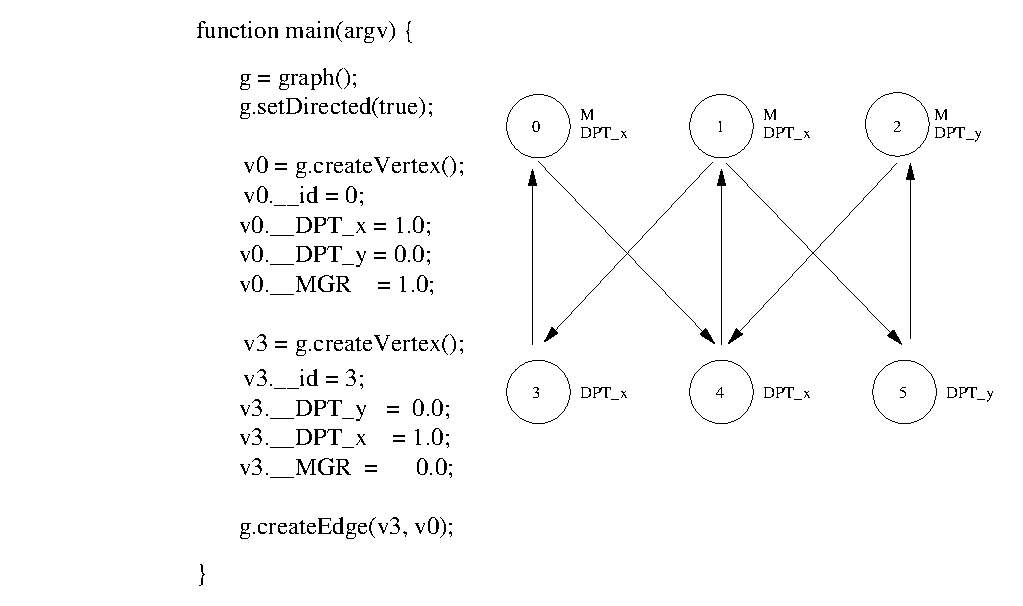
\includegraphics{Figs/1.eps}
  }
  \end{figure}
}
\frame
{
  \begin{figure}[h]
  \centering
  \scalebox{0.80}{
    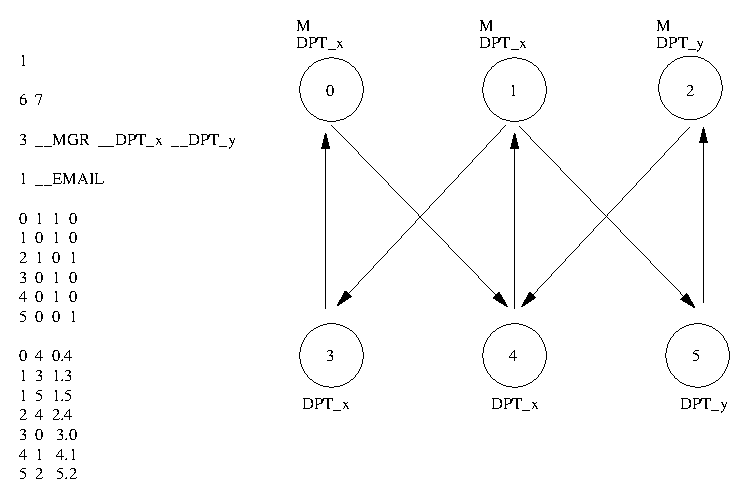
\includegraphics{Figs/2.eps}
  }
  \end{figure}
}
\frame
{
  \begin{figure}[h]
  \centering
  \scalebox{0.70}{
    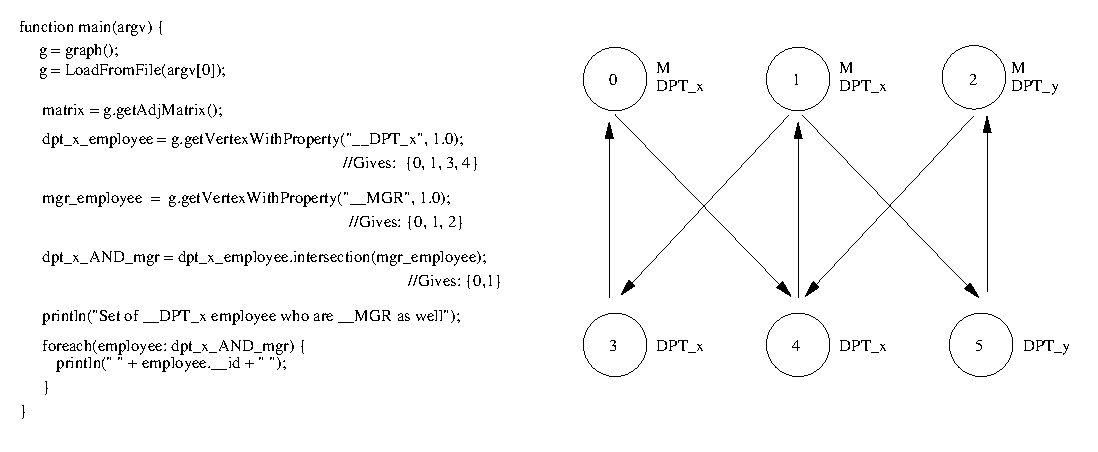
\includegraphics{Figs/3.eps}
  }
  \end{figure}
}
\frame
{
  \begin{figure}[h]
  \centering
  \scalebox{0.73}{
    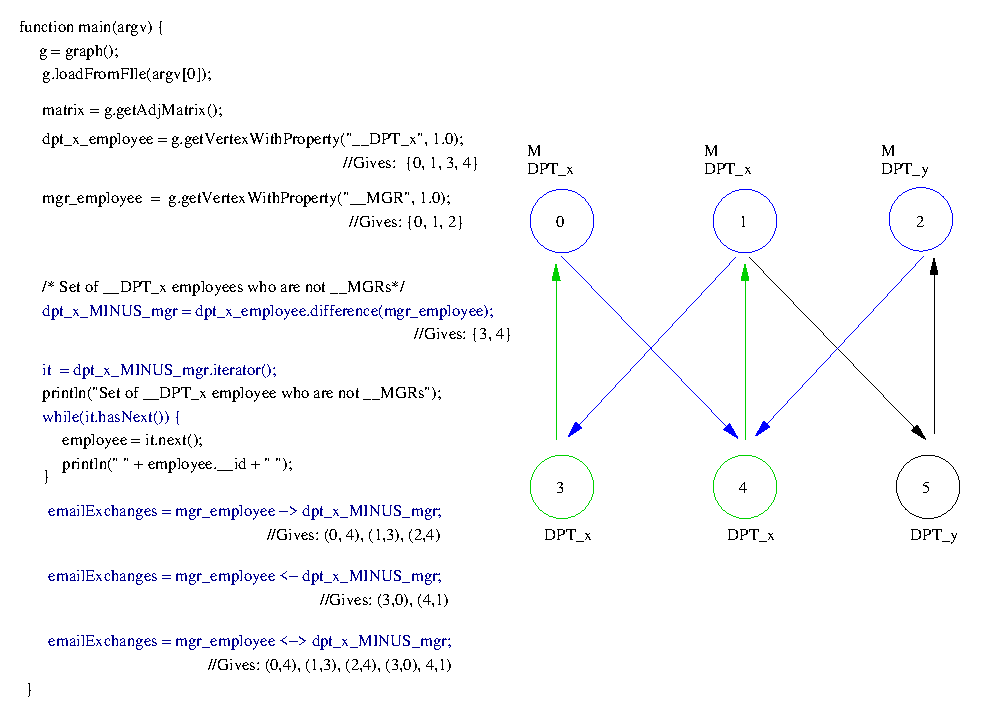
\includegraphics{Figs/4.eps}
  }
  \end{figure}
}

\frame
{
  \frametitle{\subsecname}
  \lstdfs
}

%\frame
%{
%  \frametitle{\subsecname}
%  \lstsyntax
%}

\section{Evaluation}
\subsection{Naive Implementation}
\frame
{
  \frametitle{\subsecname}
  \begin{table}[]
\centering
\caption{Slowdown of our implementation w.r.t C implementation. The graph used in all the cases consist of vertices = 500, edges = 1000. For Graph Coloring, we used the graph with vertices = 125, edges = 1000.}
\label{my-label}
\scalebox{.8} {
\begin{tabular}{|l|l|l|l|}
\hline
   \multicolumn{1}{|c|}{Algorithm}                                 & \multicolumn{1}{c|}{\begin{tabular}[c]{@{}c@{}}Fully Scripted\\ time (secs)\end{tabular}} & \multicolumn{1}{c|}{\begin{tabular}[c]{@{}c@{}}C implementation\\ time(secs)\end{tabular}} & Slowdown \\ \hline
Transitive Closure (Floyd Warshall) & 1137.40            & 4.04                   & 281.5    \\ \hline
Shortest Path (Dijkstra)            & 6.37             & 0.02                     & 318.5     \\ \hline
Minimum Spanning Tree (Prim)        & 6.34             & 0.02                      & 317.0     \\ \hline
Graph Coloring (Chaitin Optimistic) &   138.17  & 0.65                              & 212.6         \\ \hline
\end{tabular}}
\end{table}
}

\subsection{Built-in Functions}
\frame
{
  \frametitle{\subsecname}
  \begin{itemize}
    \item \tt{Graph::getAdjMatrix();}
    \item \tt{Graph::getTransitiveClosure();}
    \item \tt{Graph::getShortestPath(string wt, Vertex start, vertex end);}
    \begin{itemize}
      \item Returns the shortest distance of end from start. 
      \item Returns parent of each vertex in the shortest path tree.
      \item If \tt{end == NULL}, return the shortespath from start to all vertices.
      \item If \tt{end != NULL}, return the shortespath from start to end.
    \end{itemize} 
    \item \tt{Graph::getMST(string wt);}
    \begin{itemize}
      \item Return the parent of each vertex in the minimum snapping tree.
    \end{itemize} 
  \end{itemize}
}


\frame
{
  \frametitle{\subsecname}
  \begin{table}[]
\centering
\caption{Speedup of the our implementation with built-in functions w.r.t without using built-in functions. The graph used in all the cases consist of vertices = 125, edges = 1000}
\label{my-label}
\begin{tabular}{|l|l|l|l|}
\hline
                                    & \multicolumn{1}{c|}{\begin{tabular}[c]{@{}c@{}}With Built-ins\\ time (secs)\end{tabular}} & \multicolumn{1}{c|}{\begin{tabular}[c]{@{}c@{}}Fully Scripted\\ time(secs)\end{tabular}} & Speedup \\ \hline
Transitive Closure (Floyd Warshall) & 0.54                                                                                      & 18.19                                                                                    & 33.6    \\ \hline
Shortest Path (Dijkstra)            & 0.08                                                                                      & 0.51                                                                                     & 6.3     \\ \hline
Minimum Spanning Tree (Prim)        & 0.05                                                                                      & 0.47                                                                                     & 9.4     \\ \hline
\end{tabular}
\end{table}
}

\subsection{Revised Implementation}
\frame
{
  \frametitle{\subsecname}
  \begin{table}[]
\centering
\caption{Slowdown of our implementation w.r.t C implementation. The graph used in all the cases consist of vertices = 500, edges = 1000. For Graph Coloring, we used the graph with vertices = 125, edges = 1000.}
\label{my-label}
\begin{tabular}{|l|l|l|l|}
\hline
                                    & \multicolumn{1}{c|}{\begin{tabular}[c]{@{}c@{}}GRI\\ Time(secs)\end{tabular}} & \multicolumn{1}{c|}{\begin{tabular}[c]{@{}c@{}}C\\ Time(secs)\end{tabular}} & Slowdown \\ \hline
Transitive Closure (Floyd Warshall) & 10.26     & 4.04                               & 2.5     \\ \hline
Shortest Path (Dijkstra)            & 0.09      & 0.02                               & 4.5     \\ \hline
Minimum Spanning Tree (Prim)        & 0.09      & 0.02                               & 4.5     \\ \hline
Graph Coloring (Chaitin Optimistic) &   138.17  & 0.65                              & 212.6         \\ \hline
\end{tabular}
\end{table}

}

\end{document}
